\section{From root defect to boundary energy}\label{rec:energy}

To prove Theorem~\ref{rec:main}, we will compare the fields of the
center with their averages at the two endpoints. The following lemma
is the required calculation. It bounds the squared increases at a
chosen boundary by a quantity measured only at the root.

\begin{lemma}[Two-field energy]\label{rec:two-field}
Let $J$ be a subset of the leaves of a finite tree with root $o$. Suppose that
$P,Q,P',Q'$ are nonnegative fields, each satisfying
\[
 A_s^2\ge\sum_{c\in\operatorname{ch}(s)}A_c^2
\]
at every internal node, for each $A\in\{P,Q,P',Q'\}$. Suppose also that $P'-P=Q'-Q=d\ge0$, and
that at each internal node at least one of the inequalities for $P,Q$
is an equality. If $P_b=Q_b=0$ for $b\in J$, then
\[
 \sum_{b\in J}d_b^2
 \le\bigl[d_o(2P_o+d_o)(2Q_o+d_o)\bigr]^{2/3}.
\]
\end{lemma}

\begin{proof}
Put $E_s=[d_s(2P_s+d_s)(2Q_s+d_s)]^{2/3}$. We show that
$E_s\ge\sum_c E_c$. Suppose first that $P_s^2=\sum_cP_c^2$, and put
\[
 U_s=(P'_s)^2-P_s^2=d_s(2P_s+d_s),\qquad
 V_s=(Q'_s+Q_s)^2=(2Q_s+d_s)^2.
\]
Use the same definitions at the children. The upper inequality for
$P'$ and the equality for $P$ give $U_s\ge\sum_c U_c$. The triangle
inequality in $\ell_2$ applied to the child fields $Q',Q$ gives
$V_s\ge\sum_c V_c$. Consequently H\"older's inequality yields
\[
 \sum_c E_c=\sum_c U_c^{2/3}V_c^{1/3}
 \le\left(\sum_c U_c\right)^{2/3}
     \left(\sum_c V_c\right)^{1/3}
 \le U_s^{2/3}V_s^{1/3}=E_s.
\]
If the tight field at $s$ is $Q$, interchange $P,Q$ in this calculation.
At a leaf in $J$, $E_b=d_b^2$. Iterating the inequality through the
finite tree and discarding the nonnegative energies of the other leaves
proves the assertion.
\end{proof}

\begin{lemma}\label{rec:root-sum-stability}
Let $N=N_\Sigma$ or $N=N_J$. Suppose that $x$ is a finitely supported
unit vector and that $z\in F_H$, where $H$ is a finite initial set
containing $\supp x$. If
\[
 d=\frac12\left(\frac{N(x+z)+N(x-z)}2-1\right),
\]
then $d\ge0$ and $N(z)^3\le64d(1+d)^2$.
\end{lemma}

\begin{proof}[Proof of Lemma~\ref{rec:root-sum-stability} and the quantitative assertions of Theorem~\ref{rec:main}]
We use the fields from \eqref{rec:definition}. For a finite head vector $x$ and a finite tail $z$
vanishing on an initial set $H$ containing $\operatorname{supp}x$, set
\[
 P_s=P_s(x),\quad Q_s=Q_s(x),\quad
 P'_s=\tfrac12(P_s(x+z)+P_s(x-z)),\quad
 Q'_s=\tfrac12(Q_s(x+z)+Q_s(x-z)).
\]
The coordinate difference identity and convexity give the same
nonnegative defect $d_s=P'_s-P_s=Q'_s-Q_s$. The averaged fields satisfy
the upper inequalities by the $\ell_2$ triangle inequality. At a first
node $b$ outside $H$, the head fields vanish on its whole subtree, so
\[
 d_b=\tfrac12(P_b(z)+Q_b(z)).
\]
Only finitely many such values are nonzero. Apply
Lemma~\ref{rec:two-field} to the finite relevant part of $H$ and its
first-exit boundary, retaining at each boundary node its already-computed
full-subtree field values. Discard only subtrees where all four fields
vanish. This gives the bound on $\sum_b d_b^2$. Figure~\ref{fig:boundary}
shows the finite part through which the inequality is propagated.
\begin{figure}[tb]
\centering
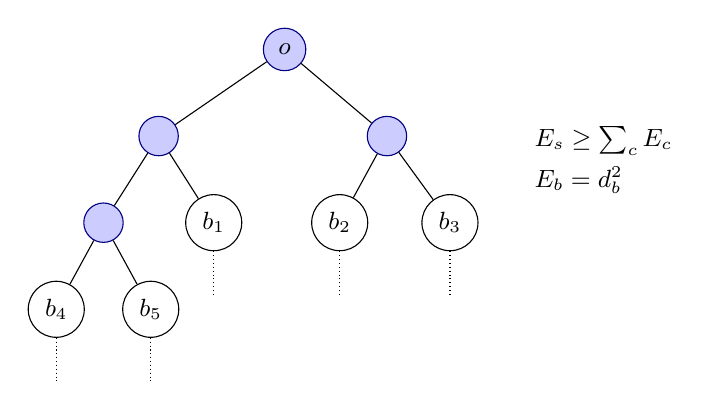
\begin{tikzpicture}[every node/.style={font=\small},
 head/.style={circle,fill=blue!20,draw=blue!50!black,minimum size=5mm},
 boundary/.style={circle,fill=white,draw=black,minimum size=5mm}]
\node[head] (o) at (0,2.2) {$o$};
\node[head] (a) at (-1.6,1.1) {};
\node[head] (b) at (1.3,1.1) {};
\node[head] (c) at (-2.3,0) {};
\node[boundary] (d) at (-0.9,0) {$b_1$};
\node[boundary] (e) at (0.7,0) {$b_2$};
\node[boundary] (f) at (2.1,0) {$b_3$};
\node[boundary] (g) at (-2.9,-1.1) {$b_4$};
\node[boundary] (h) at (-1.7,-1.1) {$b_5$};
\foreach \u/\v in {o/a,o/b,a/c,a/d,b/e,b/f,c/g,c/h}
 \draw (\u)--(\v);
\foreach \v in {d,e,f,g,h} \draw[densely dotted] (\v.south)--++(0,-.55);
\node[align=left,anchor=west] at (3.05,.8) {$E_s\ge\sum_c E_c$\\[4pt]$E_b=d_b^2$};
\end{tikzpicture}

\caption{The shaded nodes form the finite initial set $H$. Each boundary
node $b$ represents its entire descendant subtree: the head vector is zero
there, while the tail fields $P_b(z),Q_b(z)$ have already been computed.
The energy inequality propagates from these boundary values to the root.
The omitted branches contribute zero in a finite-support calculation.}
\label{fig:boundary}
\end{figure}

We next convert this energy into a norm estimate for each of the two
root conventions.
On $H$ the coordinate of $z$ is zero, so $P_s(z)=Q_s(z)$ there. With
$r_s=\max\{P_s(z),Q_s(z)\}$ one has
$r_s^2\le\sum_c r_c^2$ on $H$ and $r_b\le2d_b$ at its boundary.
Thus $r_o\le2(\sum_b d_b^2)^{1/2}$.

\emph{The sum of the root fields.} First use either root-sum space $X_\Sigma$ or $X_J$, and write
$N=N_\Sigma$ or $N=N_J$, respectively. Assume $N(x)=1$ and put
\[
 d=d_o=\frac12\left(\frac{N(x+z)+N(x-z)}2-1\right).
\]
Since $N(z)=2r_o$, the energy lemma gives
\[
 N(z)^3\le64d(2P_o+d)(2Q_o+d)\le64d(1+d)^2.
\]
The last inequality uses $P_o+Q_o=1$. The field continuity and tail
density from Proposition~\ref{rec:completion} extend this cubic inequality to
every $z\in F_H$, with the finite unit center $x$ fixed. This proves
Lemma~\ref{rec:root-sum-stability}. If $N(z)\ge t$
with $0<t<1$, then $d\ge t^3/256$: for $d\le1$ use
$(1+d)^2\le4$, and for $d>1$ the claim is immediate. Since the average
gain is $2d$, it is at least $t^3/128$.

Fix either root-sum space $X\in\{X_\Sigma,X_J\}$ with its norm $N$.
For any unit center $x_0\in X$ and $\varepsilon>0$, choose a
finite unit center $x$ with $N(x-x_0)<\varepsilon$, then choose a finite
initial $H$ containing its support. For all $y\in F_H$ with $N(y)\ge1$,
put $z=ty$ in the preceding estimate. Replacing $x$ by $x_0$ loses at
most $\varepsilon$ in the average, uniformly in $y$. Thus the supremum
over finite-codimensional subspaces at $x_0$ is at least
$t^3/128-\varepsilon$. Letting $\varepsilon\downarrow0$ and taking
the infimum over unit $x_0$ proves \eqref{rec:sum-modulus}.

\emph{The common root field.} Now use $X_0$ and write $N=N_0$,
with $o=\rho$ in the preceding calculation. By definition
$N(v)=P_o(v)=Q_o(v)$. Put
\[
 d=d_o=\frac{N(x+z)+N(x-z)}2-N(x).
\]
Now $N(z)=r_o$, and the same energy lemma yields
\[
 N(z)^3\le8d(2N(x)+d)^2.
\]
The triangle inequality gives $d\le N(z)$. For $z\ne0$ this proves the
homogeneous estimate
\[
 \frac{N(x+z)+N(x-z)}2
 \ge N(x)+\frac{N(z)^3}{8(2N(x)+N(z))^2}.
\]
The tail density from Section~\ref{rec:norms} and continuity extend
this inequality to every nonzero completed tail, proving
\eqref{rec:equal-estimate}.
\end{proof}

The factors eight and sixty-four come from the conversion of boundary
fields into the tail norm: the sum of the root fields introduces a
factor two before cubing. Both estimates therefore depend on the same
local energy inequality, while their root normalizations remain distinct.

\medskip
\noindent\emph{Remark (reciprocal form).}
In the finite-head calculation above, let $\mathcal B$ denote the
first-exit boundary, and retain the fields $P,Q$ and their averaged
increments $d$. For a node $s$ of that finite tree, put
\[
 B_s=\left(\sum_{\substack{b\in\mathcal B\\s\preceq b}}d_b^2\right)^{1/2},
 \qquad w_s^P=2P_s+d_s,\qquad w_s^Q=2Q_s+d_s.
\]
Here $s\preceq b$ means that $s$ lies on the path from the root to $b$,
including $s=b$. Both $w$ fields dominate their child Euclidean norms
and equal $d_b$ at a boundary node, so $w_s^P,w_s^Q\ge B_s$.
Applying Lemma~\ref{rec:two-field} to the descendant subtree rooted at
$s$ gives $B_s^3\le d_s w_s^P w_s^Q$. Thus, whenever $B_s>0$,
\begin{equation}\label{rec:reciprocal-energy}
 d_s\ge\frac{B_s^3}{w_s^P w_s^Q}.
\end{equation}
The undivided inequality is an equality at every boundary node.
This form expresses the same energy estimate through the accumulated
boundary norm $B_s$.
